\documentclass[12pt,titlepage]{article}
\usepackage[margin=1.25in]{geometry}
\usepackage{graphicx,amsmath,blindtext,minted}

%% Variables definition
\newcommand{\vSubject}{Basic Programming}
\newcommand{\vSubtitle}{Nested Loop Flowchart}
\newcommand{\vName}{Dicha Zelianivan Arkana}
\newcommand{\vNIM}{2241720002}
\newcommand{\vClass}{1i}
\newcommand{\vDepartment}{Information Technology}
\newcommand{\vStudyProgram}{D4 Informatics Engineering}

%% [START] Tikz related stuff
\usepackage{tikz}
\usetikzlibrary{svg.path,calc,shapes.geometric,shapes.misc}
\tikzstyle{terminator} = [rectangle, draw, text centered, rounded corners = 1em, minimum height=2em]
\tikzstyle{preparation} = [chamfered rectangle, chamfered rectangle sep=0.75em, draw, text centered, minimum height = 2em]
\tikzstyle{process} = [rectangle, draw, text centered, minimum height=2em]
\tikzstyle{decision} = [diamond, aspect=2, draw, text centered, minimum height=2em]
\tikzstyle{data}=[trapezium, draw, text centered, trapezium left angle=60, trapezium right angle=120, minimum height=2em]
\tikzstyle{connector} = [line width=0.25mm,->]
%% [END] Tikz related stuff

%% [START] Fancy header related stuff
\usepackage{fancyhdr}
\pagestyle{fancy}
\setlength{\headheight}{15pt} % compensate fancyhdr style
\fancyhead{}
\fancyfoot{}
\fancyfoot[L]{\thepage}
\fancyfoot[R]{\textit{\vSubject - \vSubtitle}}
\renewcommand{\footrulewidth}{0.4pt}% default is 0pt, overline for footer
%% [END] Fancy header related stuff

%% [START] Custom tabular command related stuff
\usepackage{tabularx}
\newcommand{\details}[2]{
    #1 & #2  \\
}
%% [END] Custom tabular command related stuff

%% [START] Figure related stuff
\newcommand{\image}[3][1]{
    \begin{figure}[h]
        \centering
        \includegraphics[#1]{#2}
        \caption{#3}
        \label{#3}
    \end{figure}
}
%% [END] Figure related stuff

\begin{document}
\begin{titlepage}
    \centering
    \vfill
    {\bfseries\LARGE
        \vSubject\\
        \vskip0.25cm
        \vSubtitle
    }
    \vfill
    
\includegraphics[width=6cm]{images/polinema-logo.png}
    \vfill
    {
        \textbf{Name}\\
        \vName\\
        \vskip0.5cm
        \textbf{NIM}\\
        \vNIM\\
        \vskip0.5cm
        \textbf{Class}\\
        \vClass\\
        \vskip0.5cm
        \textbf{Department}\\
        \vDepartment\\
        \vskip0.5cm
        \textbf{Study Program}\\
        \vStudyProgram
    }
\end{titlepage}

\subsection*{Code}
\begin{minted}[autogobble,fontsize=\small]{java}
    public class CaseStudy2 {
        public static void main(String[] args) {
            int i = 0;
            do {
                int j = 0;
                do {
                    System.out.println("*");
                    j++;
                } while (j <= i);

                System.out.println();
                i++;
            } while (i < 10);
        }
    }
\end{minted}
\subsection*{Flowchart}
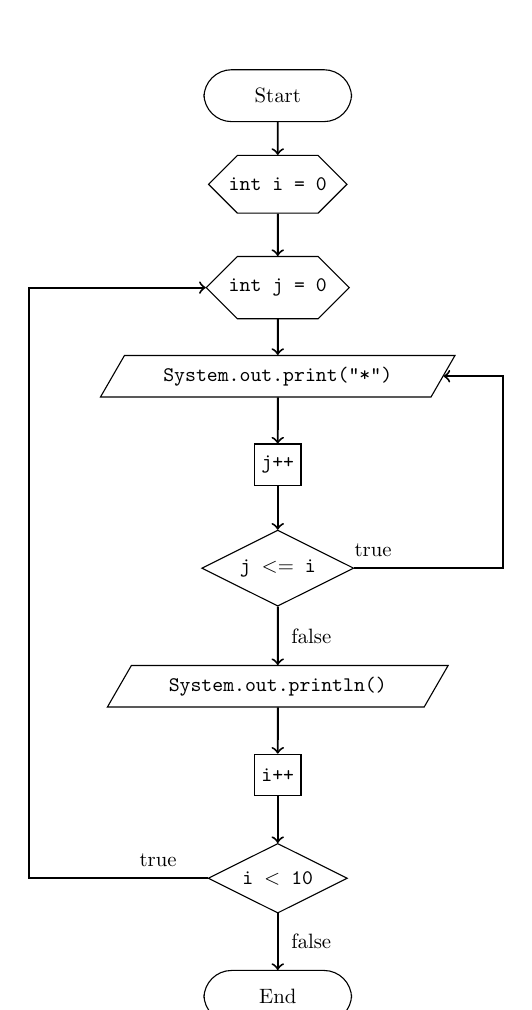
\begin{tikzpicture}[every text node part/.style={align=center}, scale=0.75, every node/.style={scale=0.75}]
    \node (start) [terminator, align=center, minimum width=2.5cm, minimum height=2.5em] {Start};
    \node (prep-i) [preparation, below of = start, yshift = -5mm] {\texttt{int i = 0}};
    \node (prep-j) [preparation, below of = prep-i, yshift = -7.5mm] {\texttt{int j = 0}};
    \node (output-star) [data, below of = prep-j, yshift = -5mm] {\texttt{System.out.print("*")}};
    \node (inc-j) [process, below of = output-star, yshift = -5mm] {\texttt{j++}};
    \node (cond-j) [decision, below of = inc-j, yshift = -7.5mm] {\texttt{j $<=$ i}};
    \node (output-line) [data, below of = cond-j, yshift = -1cm] {\texttt{System.out.println()}};
    \node (inc-i) [process, below of = output-line, yshift = -5mm] {\texttt{i++}};
    \node (cond-i) [decision, below of = inc-i, yshift = -7.5mm] {\texttt{i $<$ 10}};
    \node (end) [terminator, align=center, minimum width=2.5cm, minimum height=2.5em, below of = cond-i, yshift = -1cm] {End};
    \draw [connector] (start) -- (prep-i);
    \draw [connector] (prep-i) -- (prep-j);
    \draw [connector] (prep-j) -- (output-star);
    \draw [connector] (output-star) -- (inc-j);
    \draw [connector] (inc-j) -- (cond-j);
    \draw [connector] (cond-j) -- node[right=1mm] {false} (output-line);
    \draw [connector] (cond-j.east) -| node[above=3mm,left=1.75cm] {true} ($(output-star.east)+(1cm,0)$) -- (output-star.east);
    \draw [connector] (output-line) -- (inc-i);
    \draw [connector] (inc-i) -- (cond-i);
    \draw [connector] (cond-i) -- node[right=1mm] {false} (end);
    \draw [connector] (cond-i.west) -| node[above=3mm,right=1.75cm] {true} ($(prep-j.west)-(3cm,0)$) -- (prep-j.west);
\end{tikzpicture}

\end{document}

